<<<<<<< HEAD
%----------------------------------------------------------------------------------------
%	PACKAGES AND OTHER DOCUMENT CONFIGURATIONS
%----------------------------------------------------------------------------------------

\documentclass[10.5pt]{article}
\usepackage{graphicx}
\usepackage[utf8]{inputenc}  
\usepackage[T1]{fontenc} 
\usepackage[top=2cm,bottom=2cm,left=1.3cm,right=1.5cm,asymmetric]{geometry}
\usepackage{amsfonts}
\usepackage{graphicx}
\usepackage{caption}
\usepackage{subcaption}
\usepackage{float}
\usepackage{subfig}
%\usepackage{algorithm}
%\usepackage{algpseudocode}
\usepackage[ruled,noend]{algorithm2e}
\usepackage{fancyhdr}
\usepackage{ stmaryrd }
\usepackage{placeins}
\usepackage{ amssymb }
\usepackage{mathtools}
\usepackage{verbatim}
\usepackage{dsfont}
\pagestyle{fancy}
\renewcommand{\footrulewidth}{1pt}
\fancyhead[R]{\textit{Master MVA : Reinforcement Learning}}
\fancyfoot[L]{\textit{}}
%\usepackage{unicode-math}
%\setmathfont{XITS Math}
%\setmathfont[version=setB,StylisticSet=1]{XITS Math}
\usepackage{array,multirow,makecell}
\setcellgapes{1pt}
\makegapedcells
\newcolumntype{R}[1]{>{\raggedleft\arraybackslash }b{#1}}
\newcolumntype{L}[1]{>{\raggedright\arraybackslash }b{#1}}
\newcolumntype{C}[1]{>{\centering\arraybackslash }b{#1}}

\pagestyle{fancy}
\renewcommand{\footrulewidth}{1pt}
\fancyfoot[L]{\textit{}}

\newcommand{\argmin}{\operatorname{arg min}}

\newtheorem{definition}{Definition}
\newtheorem{theorem}{Theorem}
\newtheorem{lemma}{Lemma}
\newtheorem{corollary}{Corollary}
\newtheorem{proposition}{Proposition}

\setlength{\parindent}{0pt}
   

\begin{document}

\parskip 6pt

\begin{center}
\section*{Final project - Reinforcement Learning}
\section*{Stochastic versus adversarial bandits}
\large{Isabella Joanna Lukasewitz \& Sammy Khalife}
\end{center}

\section*{Introduction}
Multi-armed bandit games are a simple model for sequential decision making. They have been studied from the second half of the last century on and remain an important subject of research until today. The basic framework presents a player in a situation of sequential decision making. After each decision (out of a discrete and finite decision set) he receives a feedback from the environment in the form of a reward (or loss). The crucial tradeoff faced is the one between \textit{exploration} and \textit{exploitation}: While exploring the possible decision arms in order not to take suboptimal decisions, he/she should exploit what is already known in the best possible way. The performance of a strategy is usually measured as the regret with respect to a certain benchmark where the benchmark is generally given by the best fixed strategy throughout the game (to be defined more precisely in different scenarios).

For a long time, two main frameworks have been considered in the literature, largely independently from each other. The stochastic case assumes fixed underlying distributions for the respective decision arms (\cite{Thom33}, \cite{Robb52}, \cite{Auer02a}). The more general and therefore more difficult adversarial case (\cite{Auer95},  \cite{Auer02b}) does not make such an assumption. Rewards are assumed to be generated entirely randomly and fully determined given a sequence of decisions ahead of the game (which is obviously unknown to the player).

For both scenarios, algorithms have been developed with nearly optimal worst-case guarantees. In a stochastic environment, the UCB1 algorithm (\cite{Auer02a}) for instance attends a regret of $O(\log n)$ while in the adversarial case, $O(\sqrt{n})$ is reached by EXP3 (\cite{Auer02b}) for bounded rewards. However, generally algorithms designed for the stochastic framework fail completely in the adversarial one while algorithms adapted to the adversarial framework do not manage to take advantage of the "nice" stochastic case. Moreover, no regimes different from the "extreme" adversarial and stochastic ones had been considered.

Attempts to combine the two have been made only recently. In this article, we aim to present them briefly, put them into context and analyze their performance. For this end, we will first provide a short overview of the basic main algorithms considered until today, their performance and their regret guarantees. In the second part, we will analyze more closely two algorithms proposed for the two frameworks jointly, the SAO algorithm (Bubeck et al., 2012 \cite{Bube12}) and the so-called EXP3++ (Seldin et al, 2014 \cite{Seld14}). Finally, we will present an algorithm that was introduced recently by Sani et al. \cite{Sani14}. It has been developed for a more general  online decision problem with full feedback. We will adapt it to the bandit framework and test its performance therein. All the numerical results can be found together in the last section.

\section*{Multi-armed bandit environments}
Let $r_{t}^{A_{t}}$ be the reward obtained at time $t$ by pulling arm $A_{t}$. We will consider four different environments, following in that Seldin et al. \cite{Seld14}. In all cases, rewards are assumed to be bounded in $[0,1]$. The expected regret to be minimized is a priori defined as the difference between the expected loss of the algorithm up to round $t$ and the expected loss of the best arm up to round $t$:
$$\mathbb{E}[R(t)]=\max_{a}\{ \sum_{s=1}^{t} \mathbb{E}[r_{s}^{a}]\}-\sum_{s=1}^{t} \mathbb{E}[r_{s}^{A_{s}}].$$
The expectation is taken over the possible randomness of the algorithm and loss generation model. 

In the \textbf{adversarial regime}, the rewards are generated by an ''unrestricted adversary'' (oblivious to the algorithm's actions). This is the most general case. The regret is a posteriori computed as the difference to the best fixed strategy in hindsight: 
$$ R(t)=\max_{a}\{ \sum_{s=1}^{t} r_{s}^{a} \}-\sum_{s=1}^{t} r_{s}^{A_{s}}.$$

In the \textbf{stochastic regime}, we suppose that the rewards are sampled independently with respect to a stationary distribution. Then $\mathbb{E}[r_{s}^{a}]=\mu_{a}$, and the regret simplifies : 
$$\mathbb{E}[R(t)]=t\max_{a}\mu_{a}-\sum_{s=1}^{t} \mathbb{E}[r_{s}^{A_{s}}],$$
which can be written as
$$\mathbb{E}[R(t)]=\sum_{a}\mathbb{E}[N_{t}(a)]\Delta_{a}$$ 
where $\Delta(a)=(\max_{a'}\mu_{a'})-\mu_{a}$ and $N_{t}(a)$ is the number of times $a$ has been pulled until time $t$.

This are the two classical framework as described in the beginning, stated in their most simple and original form. Furthermore, Seldin et al. introduce two new ones that can be regarded as in between the aforementioned ones and will be referred to later in this article.

The first of them is called \textbf{adversarial regime with a gap}, which is an adversarial regime for which we suppose that there exists a round $\tau$ and an arm $a_{\tau}*$ such that for any $t \geq \tau$, $a_{\tau}*$ persists to be the best arm in hindsight for all rounds $t \geq \tau$, i.e $\forall \, t \geq \tau$,  $a_{\tau}* \in \argmin_{a'}(\sum_{s=1}^{t}l_{s}^{a'})$.

The \textbf{contamined stochastic regime} is a stochastic regime with adversarial elements. The adversary chooses some pairs $(t,a)$ (''locations'') before the game starts and assigns their rewards in an arbitrary way. The rest of the rewards are generated as in the stochastic framework.

\section*{Popular bandit algorithms - a selection}

In this section we will give a short overview of the algorithms treated in class and compare their regret bounds. Since a lot of this material has been already treated throughout the course, we will keep the presentation short. Please note that the numerical comparison will take place in the last section.

\subsection*{Stochastic framework}

The stochastic framework was the first one to be treated in multi-armed bandit problems. The Thompson algorithm, a very efficient algorithm for problems following the stochastic assumption, was already proposed in 1933 (it had to be rediscovered many decades later, however) \cite{Thom33}. 

In 1985, Lai et al. proved in \cite{Lai85} an asymptotic lower bound of the order of $\log n$. The significance is such that no algorithm can consistently achieve an asymptotic expected worst-case regret in the stochastic environment that is of an order better then $O(\log n)$:
\begin{theorem}
Under the assumptions of the stochastic regime, the sampling expectation of the single arms is asymptotically lower bounded by
$$ \lim \sup_n \frac{\mathbb{E}N_{t}(a)}{\log n} \geq \frac{1}{KL ( \nu_k || \nu^*)} $$
where $KL$ denotes the Kullback-Leibler divergence: $KL(\nu || \nu') = \int d \nu \log (d \nu / d \nu ' )$. Therefore,
$$ \mathbb{E}R_n = O(\log n).$$
\end{theorem}

Since then, researchers have been trying to develop algorithms whose regret guarantees are as close as possible to this lower bound (while noting that the statement is only asymptotic and therefore not perfectly adapted to the finite-time setting). A very popular basic algorithm, the UCB algorithm, was proposed by Auer et al. in \cite{Auer02a}. It is commonly called an "optimistic" algorithm since it does not only compute an estimate of the expected rewards, but rather an upper-confidence bound UCB (called an "index" of a given arm), and the agent's choice is an arm with highest UCB. Its regret is of the order of $\log n$, the constants being given by:
\begin{theorem}
The expected regret of the UCB algorithm is bounded as
$$ \mathbb{E}[R(t)] = \sum_{a}\mathbb{E}[N_{t}(a)]\Delta_{a} <
 6 \sum_{a: \, \Delta_a > 0} \frac{\log t}{\Delta_a} + K (\frac{\pi^2}{3} + 1).$$
\end{theorem}

UCB has been extended numerous times (e.g. \cite{Audi09}, \cite{Audi10}). While the constants could be improved in many cases, it also has to be noted that these bounds give a worst-case guarantee and algorithms may behave very differently from each other in different scenarios, despite having similar bounds.

One extension is given by the KL-UCB algorithm. It is still index-based, however it uses slightly more complex upper confidence bounds that are based on the KL divergence of Bernoulli variables. Since it consistently performs better than UCB, we cite the regret bound from \cite{Gari11}, Garivier et al. in the appendix.

The aforementioned Thompson Sampling follows a different mindset. It is based on Bayesian ideas of the underlying distributions of the arms. It does achieve a very competitive regret, however. It's general problem dependent and independent regret bounds have only been derived very recently in \cite{}. We cite their two main results.

\begin{theorem}
For the $K-$armed stochastic bandit problem, Thompson Sampling algorithm has expected regret
$$\mathbb{E}[R(t)] \leq (1 + \epsilon) \sum_{i=1}^N \frac{\log t}{d(\mu_i, \mu_1)}\Delta_i + O(\frac{K}{\epsilon^2} $$
in time $t$ where $d(\mu_i, \mu_1) = \mu_i \log \frac{\mu_i}{\mu_1} + (1 - \mu_i) \frac{1-\mu_i}{1 - \mu_1}$.
Furthermore,
$$ \mathbb{E}[R(t)]  \leq O(\sqrt{K t \log t}$$.
\end{theorem}

\subsection*{Adversarial framework}

The adversarial framework encompasses the stochastic one, but also much more difficult cases. A regret bound of the order of $\log n$ can hence not be established. On the contrary, it has been shown that independently of the algorithm used, there can always be found a case where the regret will be of the order of $\sqrt(n)$ (see e.g. \cite{Cesa06}):
$$\underset{\inf}{\text{alg}} \sup_{\text{prob}} \; R_n = \Omega(\sqrt{nK}).$$

The so-called EXP3 algorithm plays a similar role in this adversarial environment as UCB does in the stochastic one. It has been introduced in 2002 by Auer et al. \cite{Auer02b} and has been equally subject to some extensions. The authors showed that its regret matches the order of the general bound mentioned above:
\begin{theorem}
If EXP3 is run with $\gamma = \eta$, then it achieves a regret
$$ R_n(\mathcal{A}) = \max_{i = 1,...,N} \sum_{t=1}^n X_{i,t} - \mathbb{E} \left [ \sum_{t=1}^n X_{I_t,t}\right]
\leq (e-1)\gamma G_{\text{max}} + \frac{N \log N}{\gamma}$$
with $G_{\text{max}} = \max_{i = 1,...,N} \sum_{t=1}^n X_{i,t}$. If EXP3 is run with 
$$ \gamma = \eta = \sqrt{\frac{N \log N}{(e-1)n}}, $$
then it achieves a regret
$$ R_n(\mathcal{A}) \leq O(\sqrt{n N \log N}).$$
\end{theorem}

The EXP3.P was equally proposed in \cite{Auer02b}. It is a version of the EXP3 algorithm that introduces a biased estimate of the cumulative gain and exhibits advantageous theoretical properties when deriving high-probability bounds. They obtain therefore for this framework a bound on the actual regret (not in expectation) that holds with a certain probability which is linked to the parameters of the algorithm.
\begin{theorem}
If EXP3.P is run with parameters in the ranges
$$\gamma \leq \frac{1}{2}; \quad 0 \leq \eta \leq \frac{\gamma}{2N}; \quad \sqrt{\frac{1}{nN}\log \frac{N}{\delta}} \leq \beta \leq 1 $$
then it achieves a regret 
$$R_n^{HP}(\mathcal{A}) \leq n(\gamma + \eta(1+\beta)N) + \frac{\log N}{\eta} + 2nN\beta $$
with probability at least $ 1 - \delta$.
If EXP3.P is run with parameters in the ranges
$$ \beta = \sqrt{\frac{1}{nN}\log \frac{N}{\delta}}; \quad \gamma = \frac{4N\beta}{3 + \beta}; \quad \eta = \frac{\gamma}{2N} $$
then it achieves a regret
$$ R_n^{HP} (\mathcal{A}) \leq \frac{11}{2} \sqrt{nN \log (N/\delta)} + \frac{\log N}{2}$$
with probability at least $1 - \delta$. 
\end{theorem}

Even if this section - due to the limited scope of this paper - ressembles rather a list of convergence bounds than an in-depth analysis of the individual algorithms, it still points out the general framework of bandit problem analysis. Sufficiently simple algorithms have been found whose theoretical performance - at least in the expected worst-case - is nearly as good as it can become, within the division of the field into adversarial and stochastic problems. These algorithms are practical and widely applied. However, what has become clear in the course of the trimester and will be further pointed out in the numerical section, they are not only theoretically, but also practically not adapted to the exploitation of the respectively other framework. On the other hand, in praxis one often cannot know exactly which type of regime one is in and most of the times they may be mixed, not assuming any of the "pure" cases. Attempting to bridge this gap is therefore a very natural next step in the analysis of bandit problems.

\section*{"The best of both worlds": The SAO algorithm}

There has only been very recently attempts to overcome the distinction between the two aforementioned frameworks. The first one was made by Bubeck et al. in 2012 \cite{Bube12}, where they introduced the so-called SAO algorithm. This algorithm manages in a certain way to combine the two initial scenarios: It has a build-in mechanism to detect the framework the player is in. However, it does not explicitly leave room for scenarios that are not purely stochastic or purely non-stochastic. This further extension will be tackled by the EXP3++ algorithm in the following section.

The SAO algorithm starts off with classical ideas for the stochastic framework, interleaving an \textit{exploration} and an \textit{exploitation} phase. At the beginning, all arms are activated and are sampled with the same probability. In the course of the algorithm, more and more arms get gradually deactivated (their sampling probability decreases smoothly) and the remaining arms are sampled with steadily increasing probability. The algorithm thus moves gradually from an exploration to an exploitation strategy. At each point in time, certain consistency conditions are checked to ensure that the assumed stochastic framework holds. As soon as one of these conditions fails, the algorithm assumes an adversarial framework and switches to the EXP3.P algorithm described in the previous section. 

An an important novelty, they mange to prove an $\tilde{O}(\sqrt{n})$ regret bound for the adversarial case and a $polylog(n)$ bound for the stochastic case, thus coming close to the theoretical performance bounds for the UCB and the EXP3 algorithm that we recalled in the previous section. Their main result reads as follows:
\begin{theorem}
There exists an algorithm SAO for the MAB problem such that:
\begin{enumerate}
\item[(a)] in the adversarial model, SAO achieves regret $\mathbb{E}[R_n] \leq O(\sqrt{nK} \log^{3/2}(n) \log K)$.
?\item[(b)] in the stochastic model, SAO achieves regret $\mathbb{E}[R_n] \leq O(K \log^{2}(n) \log K)$.\end{enumerate}
\end{theorem}

The details are stated in the following theorem. The algorithm (with the explanation of the parameters) can be found in \cite{Bube12}.
\begin{theorem}
SAO with $\beta = n^4$ satisfies in the stochastic model:
$$ \mathbb{E}[R_n] \leq O \left (\frac{K \log(K) \log^2(n)}{\Delta} \right),$$
and in the adversarial model:
$$\mathbb{E}[R_n] \leq O(\log(K) \log^{3/2}(n) \sqrt{nK}).$$
More precisely, for any $\delta \in (0,1)$, with probability at least $1-\delta$, SAO with $\beta = 10Kn^3 \delta^{-1}$ satisfies in the stochastic model:
$$\bar{R}_n = \frac{260K (1 + \log K) \log^2(\beta)}{\Delta},$$
and in the adversarial model:
$$R_n = \leq 60(1 + \log K) (1 + \log n) \sqrt{nK \log(\beta) + 5 K^2 \log^2(\beta)} + 200K^2 \log^2(\beta).$$
\end{theorem}

We have tested the performance of the algorithm in comparison to several standard algorithms that were brought up in the last section. To our knowledge, this has not been done before. This may well be due to the fact that Bubeck et al. state themselves - a practical implementation of the algorithm should encompass some enhancements like an extension to a mixed stochastic-adversarial environment and the result is more of a theoretical interest. As expected, the performance does therefore not quite match the one of the benchmarks. In several examples, we can see however how the algorithm actually manages to bridge the gap better than the current standard. In any case, it is to be noted that the theoretical value of this algorithm is valid since it introduces for the first time theoretical guarantees for the fact that it is possible to tackle both environments at the same time with guarantees that respectively nearly meet the ones of current standard algorithms. This had not been clear a priori and opened a wide range of improvement options.

\section*{EXP3++: An adapted EXP3 algorithm}

Finally, Seldin et al. recently proposed an algorithm that seems to tackle a lot of the problems in a quite promising way (\cite{Seld14}). In particular, they manage to derive bounds for contaminated regimes that are neither purely stochastic nor purely non-stochastic, which had seemingly not been done before. Furthermore, they do not require any knowledge about the time horizon as does SAO.

EXP3++ (see algorithm \ref{EXP++} in the appendix) is based on a rather straightforward extension of EXP3, the popularity and simplicity of which make it rather likely for the former to incite a range of applications and enhancements. The main novelty that is introduced in the algorithm is a set of time-dependent exploration parameters $\xi_t(a)$ that complete the learning rate $\eta_t$. The EXP3 algorithm (see algorithm \ref{EXP3} in the appendix) is a special case of the EXP3++ algorithm with $\xi_t(a) = 0$ and $\eta_t = 2 \beta_t$, which illustrates the change.

The authors show that running only the learning rate $\eta_t$ suffices to control the regret of \text{EXP3++} in the adversarial regime, irrespective of the choice of the exploration parameters. On the other hand, tuning the exploration parameters suffices to control the regret of EXP3++ in the stochastic regime as long as $\eta_t \geq \beta_t$. Optimizing the parameters jointly, they obtain an optimal regret in the adversarial regime ($O(\sqrt{n})$) and a nearly optimal $polylog(n)$ regret in the stochastic regime. Furthermore, they derive control bounds even in the two interlinked regimes (contaminated stochastic regime and adversarial regime with a gap) they introduced.

\subsection*{Adversarial regimes}

\begin{theorem}
For $\eta_{t}=\beta_{t}$ and $\xi_t(a) \geq 0$, the regret for any $t\geq0$ satisfies 
$$R(t) \leq 4\sqrt{K t\ln K}.$$ 
\end{theorem}
This regret bound is just a factor of 2 worse than the regret of EXP3 with losses.

\subsection*{Stochastic regime}
If the gaps between the individual arms are known, $\xi_{t}$ and $\eta_{t}$ can be tuned to control the regret. Since in practice, this is usually not the case, an empirical estimator will be used:
$$\hat{\Delta}_{t}(a)=min\{1,\frac{1}{t}(\max_{a'}(\tilde{L}_{t}(a')-\tilde{L}_{t}(a))\}$$
\begin{theorem}
Knowing the gaps $\Delta(a)$, with $\xi_{t}(a)=\frac{c\ln(t\Delta(a)^{2})}{t\Delta(a)^{2}}$, the regret satisfies :
$$R(t) \leq \sum_{a} O(\frac{\ln(t)^{2}}{\Delta(a)})+\sum_{a}\tilde{O}(\frac{K}{\Delta(a)^{3}})$$
\end{theorem}

\begin{theorem} \label{stoch}
Let us consider the empirical gap $\Delta_{t}(a)$ defined previously, a time $t^{*}$ such that $t^{*}\geq \frac{4c^{2}K\ln(t*)^{4}}{\ln(K)}$ and let $t^{*}(a)=max\{t*,\lceil e^{1/\Delta(a)^{2}}\rceil\}$.
Then by tuning $\xi_{t}(a)=\frac{c\ln(t)^{2}}{t\hat{\Delta}_{t-1}(a)^{2}}$ (termed EXP3$++^{AVG}$ algorithm) the regret in the stochastic regime satisfies :
$$R(t) \leq \sum_{a}O(\frac{\ln(t)^{3}}{\Delta{a}})+\sum_{a}\Delta(a)t^{*}(a)$$
\end{theorem}

\subsection*{Contaminated stochastic regime}

\begin{theorem}
With the same assumptions as in theorem \ref{stoch} except that $t^{*}(a)=max\{t^{*}, \lceil e^{4/\Delta(a)^{2}}\rceil \}$, the regret satisfies :
$$R(t) \leq \sum_{a}O(\frac{\ln(t)^{3}}{\Delta(a)})+\sum_{a}max\{t^{*}(a),\tau\}$$

\subsection*{Adversarial regime with a gap}
\textbf{Theorem 5} With the same assumptions as in theorem \ref{stoch}, the regret satisfies :
$$R(t) \leq \sum_{a}\{\min_{\tau}\{max\{t^{*},\tau,e^{1/(\Delta(\tau,a))^{2}}\}+O(\frac{\ln(t)^{3}}{\Delta(\tau,a)})\}$$
\end{theorem}

Both theory and practice show that parameter tuning is crucial. With $\eta_{t}=\beta_{t}$, the EXP3++ algorithm provides a guarantee against adversarial situations. On the other hand, a configuration such that $\eta=1$ provides better results in a stochastic regime. The authors see a considerable potential for a better exploitation of the algorithm in an optimized tuning of this parameters.

In the numerical section we will see that similar to the results the authors get, the EXP3++ algorithm does seem to represent a competitive practical alternative to existing algorithms, which is not the case for SAO. Nevertheless, a favorable parameter adjustment does require a certain knowledge about the given environment.


\section*{The $(\mathcal{A},\, \mathcal{B})-$PROD algorithm applied to multi-armed bandits}

The multi-armed bandit problem can be seen as a special case of a general online decision-making problem. It belongs to the class of partial feedback problems: In an MAB, the player's feedback is equal to his reward. He does in particular not obtain any knowledge regarding the theoretical rewards of the arms he has not played.

In general decision-making problems, the player receives a more comprehensive feedback. One notably assumes that he has access to the reward he would have received had he taken a different decision.

The question discussed in this paper - essentially of how to construct an algorithm that has both worst-case guarantees against "hard" cases and while still being able to take advantage of "easy" cases - can obviously be posed in all kinds of different scenarios and is of a much more general interest than only in the case of MABs. It has been discussed to a much greater extent already in online learning than in the case of MABs, of which we have just outlined the first attempts.

In this context, Sani et al. \cite{Sani14} proposed an algorithm recently that aims at achieving exactly that. Their $(\mathcal{A},\, \mathcal{B})-$PROD algorithm is designed to assume the worst-case guarantee bound from an algorithm that is generally adapted to "hard" cases while staying within a constant factor of a benchmark. It can for example take two methods $\mathcal{A}$ and $\mathcal{B}$ as input where $\mathcal{A}$ provides the robustness to difficult problems while $\mathcal{B}$  takes advantage of the easy ones. $(\mathcal{A},\, \mathcal{B})-$PROD then follows either the one or the other input algorithm in its prediction, depending on weights that are shaped by the game history.

In the original paper, the weight update requires the knowledge of the rewards of both the $\mathcal{A}$ and the $\mathcal{B}$ algorithm. In the MAB setting, this is not given. In order to account for that, an importance weighting update can be used. We have implemented two versions: In the first one, $\mathcal{A}$ and $\mathcal{B}$  are updated with the arm they chose and and are accorded a zero reward if this arm had not been played in the end. In the second one, both algorithms are updated with the pair of (action, reward) that was eventually chosen. Please refer to the algorithms \ref{Prod1} and \ref{Prod2} in the appendix for the exact algorithm formulations.

Having implemented both versions, we see that (as it is more intuitive) version 2 of the algorithm always outperforms version 1. In terms of the input algorithms, we have implemented the method for $\mathcal{A} $ as the EXP3 algorithm and $\mathcal{B}$ as UCB and Thompson Sampling. Whether the algorithms performs better with UCB or Thompson sampling, depends on the problem. In general however, the algorithm performs better or about as good as any benchmark algorithm. The results can be found in the next section in direct comparison to the other algorithms. 

\section*{Numerical experiments}

In all of the experiments (unless stated otherwise) we take the mean over 500 simulations. We tried to choose good parameters for each case. However, parameters could have been optimized even more. We are nevertheless confident that our results give a good idea of the general performance of the algorithms.

\subsection*{Stochastic environment}

\begin{figure}[H]
\minipage{0.33\textwidth}
  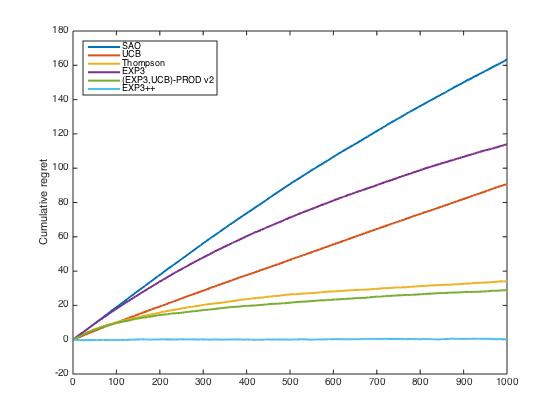
\includegraphics[width=\linewidth]{Stoch1_mix.jpg}
  \subcaption{Algorithm performances}\label{fig:awesome_image1}
\endminipage\hfill
\minipage{0.33\textwidth}
  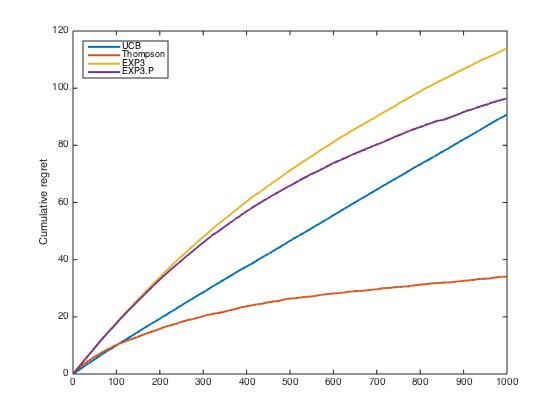
\includegraphics[width=\linewidth]{Stoch1_old.jpg}
  \subcaption{Standard algorithms}\label{fig:awesome_image2}
\endminipage\hfill
\minipage{0.33\textwidth}%
  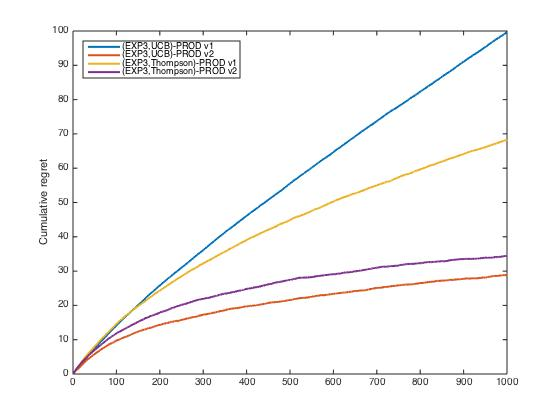
\includegraphics[width=\linewidth]{Stoch1_prod.jpg}
  \subcaption{$(\mathcal{A},\, \mathcal{B})-$PROD for multiarmed bandits}\label{fig:awesome_image3}
\endminipage
\caption{An easy stochastic problem with 5 arms, different distributions}
\end{figure}

\begin{figure}[H]
\minipage{0.33\textwidth}
  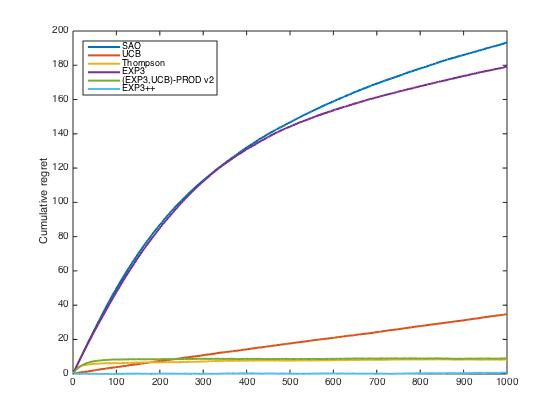
\includegraphics[width=\linewidth]{Stoch2_mix.jpg}
  \subcaption{Algorithm performances}\label{fig:awesome_image1}
\endminipage\hfill
\minipage{0.33\textwidth}
  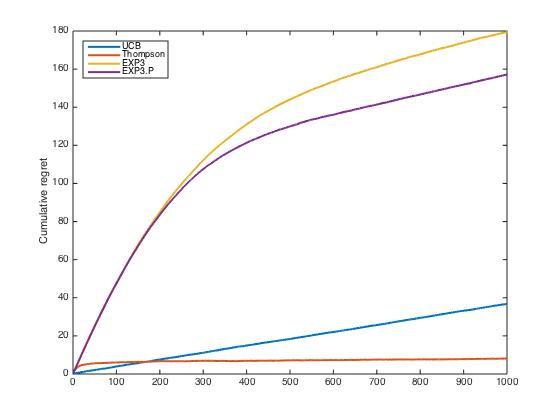
\includegraphics[width=\linewidth]{Stoch2_old.jpg}
  \subcaption{Standard algorithms}\label{fig:awesome_image2}
\endminipage\hfill
\minipage{0.33\textwidth}%
  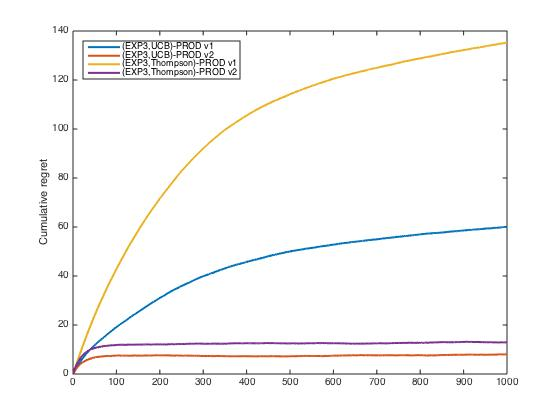
\includegraphics[width=\linewidth]{Stoch2_prod.jpg}
  \subcaption{$(\mathcal{A},\, \mathcal{B})-$PROD for multiarmed bandits}\label{fig:awesome_image3}
\endminipage
\caption{An easy Bernoulli problem with 4 arms, $KL = 1.5499$}
\end{figure}

\begin{figure}[H]
\minipage{0.33\textwidth}
  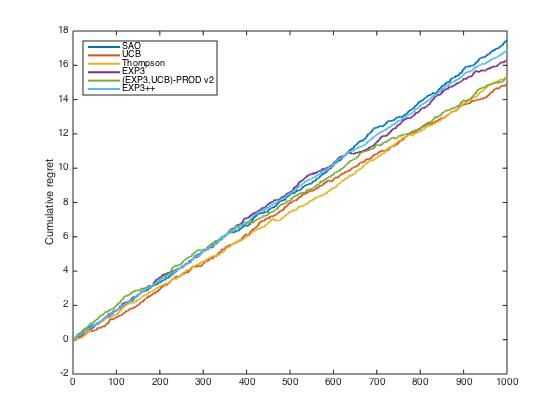
\includegraphics[width=\linewidth]{Stoch3_mix.jpg}
  \subcaption{Algorithm performances}\label{fig:awesome_image1}
\endminipage\hfill
\minipage{0.33\textwidth}
  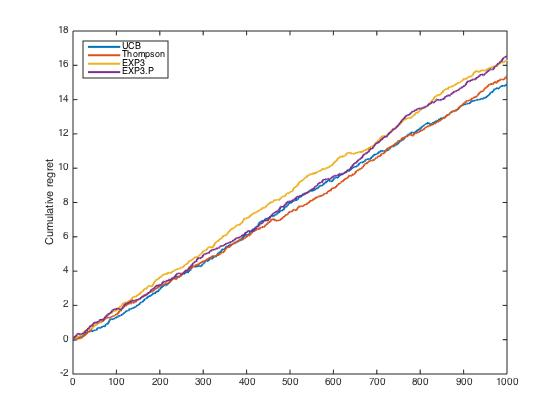
\includegraphics[width=\linewidth]{Stoch3_old.jpg}
  \subcaption{Standard algorithms}\label{fig:awesome_image2}
\endminipage\hfill
\minipage{0.33\textwidth}%
  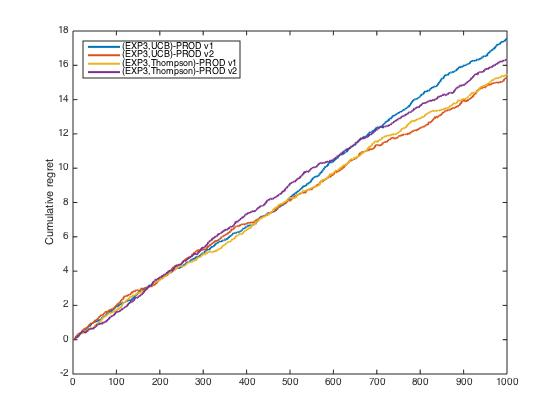
\includegraphics[width=\linewidth]{Stoch3_prod.jpg}
  \subcaption{$(\mathcal{A},\, \mathcal{B})-$PROD for multiarmed bandits}\label{fig:awesome_image3}
\endminipage
\caption{A difficult Bernoulli problem with 9 arms, $KL = 259.1457$}
\end{figure}

With respect to the standard algorithms, we see the the classical picture: UCB and Thompson sampling perform well on the stochastic cases, EXP3 and EXP3.P do not. It is to be noted, however, that EXP3.P performs consistently better than EXP3. Thompson sampling is especially efficient for easy Bernoulli problems. For difficult problems, the differences between the algorithm performances diminish.

For the new algorithms, EXP3++ seems very competitive while SAO is not necessarily adapted to a practical implementation. The $(\mathcal{A},\, \mathcal{B})-$PROD algorithm is a very positive surprise: While version 1 generally fails, version 2 performs very well. For the stochastic problems, UCB usually performs slightly better as $\mathcal{B}$ than Thompson Sampling. Interestingly, the (EXP3,UCB)-PROD algorithm usually matches the Thompson sampling performance.

\subsection*{Adversarial environment}

\begin{figure}[H]
\minipage{0.33\textwidth}
  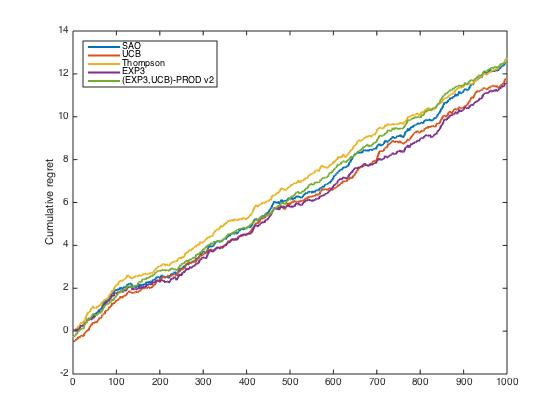
\includegraphics[width=\linewidth]{Adv1_mix.jpg}
  \subcaption{Algorithm performances}\label{fig:awesome_image1}
\endminipage\hfill
\minipage{0.33\textwidth}
  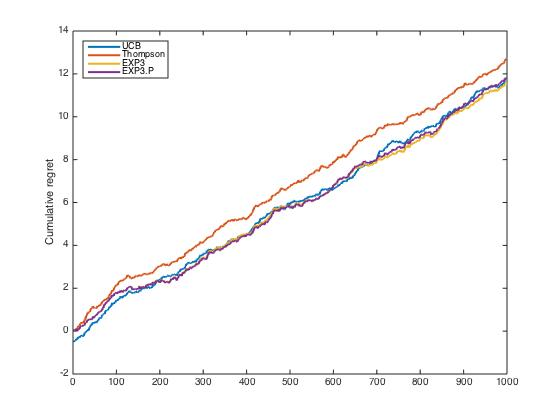
\includegraphics[width=\linewidth]{Adv1_old.jpg}
  \subcaption{Standard algorithms}\label{fig:awesome_image2}
\endminipage\hfill
\minipage{0.33\textwidth}%
  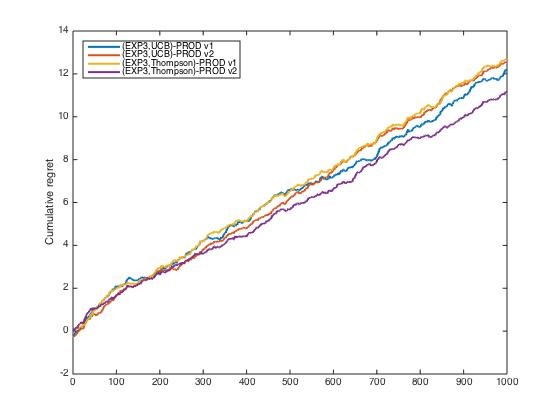
\includegraphics[width=\linewidth]{Adv1_prod.jpg}
  \subcaption{$(\mathcal{A},\, \mathcal{B})-$PROD for multiarmed bandits}\label{fig:awesome_image3}
\endminipage
\caption{A small adversarial problem with 2 arms}
\end{figure}

In the given adversarial problem, differences between algorithm are less prominent. However, EXP3 performs better than UCB and Thompson Sampling. SAO is mildly competitive, $(\mathcal{A},\, \mathcal{B})-$PROD performs very well.

\subsection*{Adversarial environment with a gap}

\begin{figure}[H]
\minipage{0.33\textwidth}
  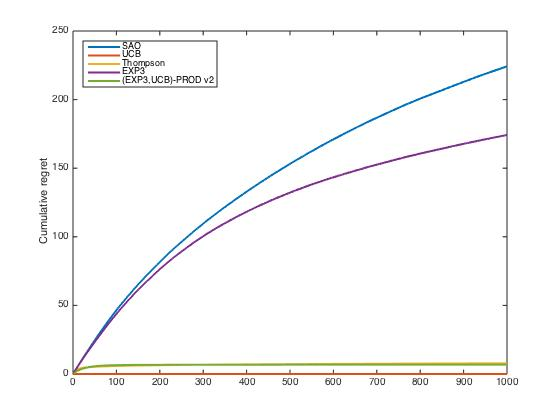
\includegraphics[width=\linewidth]{Adv2_mix.jpg}
  \subcaption{Algorithm performances}\label{fig:awesome_image1}
\endminipage\hfill
\minipage{0.33\textwidth}
  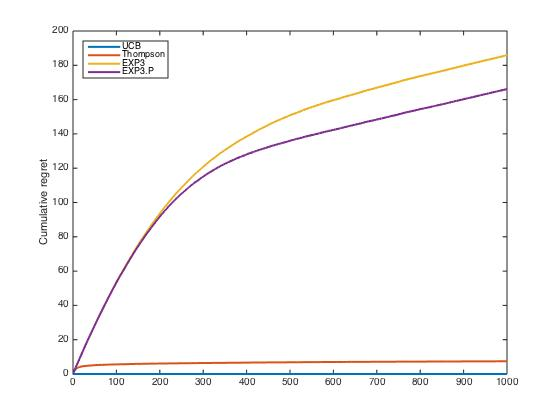
\includegraphics[width=\linewidth]{Adv2_old.jpg}
  \subcaption{Standard algorithms}\label{fig:awesome_image2}
\endminipage\hfill
\minipage{0.33\textwidth}%
  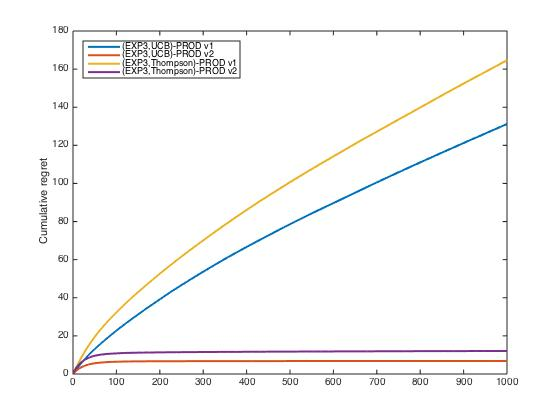
\includegraphics[width=\linewidth]{Adv2_prod.jpg}
  \subcaption{$(\mathcal{A},\, \mathcal{B})-$PROD for multiarmed bandits}\label{fig:awesome_image3}
\endminipage
\caption{An adversarial problem with one unique best arm}
\end{figure}

In this environment, all arms are (truly) adversarial, but there exists a gap to a single best arm. This gap leads the algorithms into a performance very similar to the stochastic framework.

\subsection*{Contaminated stochastic regime}

\begin{figure}[H]
\minipage{0.33\textwidth}
  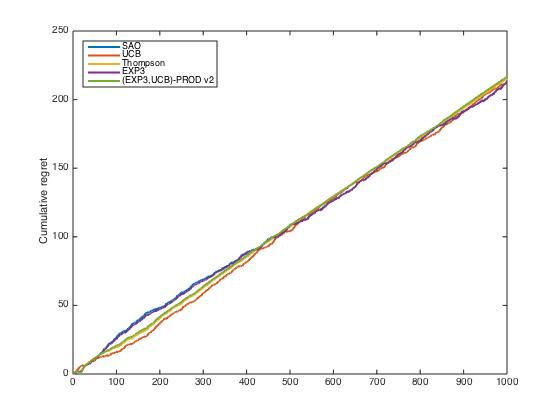
\includegraphics[width=\linewidth]{CStoch_mix.jpg}
  \subcaption{Algorithm performances}\label{fig:awesome_image1}
\endminipage\hfill
\minipage{0.33\textwidth}
  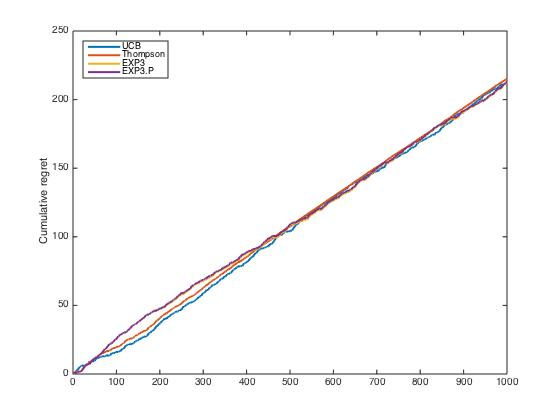
\includegraphics[width=\linewidth]{CStoch_old.jpg}
  \subcaption{Standard algorithms}\label{fig:awesome_image2}
\endminipage\hfill
\minipage{0.33\textwidth}%
  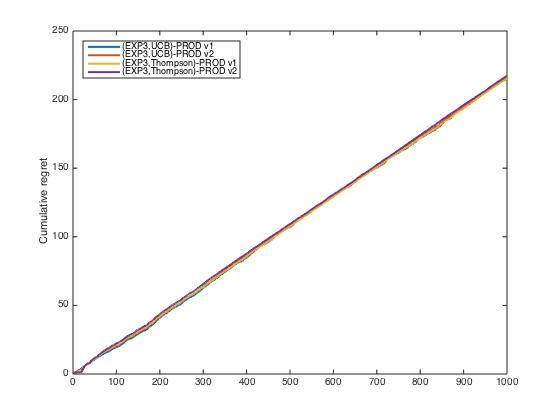
\includegraphics[width=\linewidth]{CStoch_prod.jpg}
  \subcaption{$(\mathcal{A},\, \mathcal{B})-$PROD for multiarmed bandits}\label{fig:awesome_image3}
\endminipage
\caption{A contaminated stochastic regime with 5 adversarial arms and 5 rather difficult Bernoulli arms}
\end{figure}

Interestingly, in this given problem the compilation of stochastic and adversarial arms further approached the performance of the algorithms to each other and made them behave like in an adversarial framework. This picture would have to be explored on a wider set of examples.

\subsection*{An EXP3++ discussion}
We would like to further highlight the EXP3++ performance with the help of the following examples since part of them gives results that differ from the ones obtained on the examples of the previous section. The implementation uses a time-depending gap $$\Delta(t,a)=\max_{a}(\mathbb{E}[r_{t}^{a}]-\mathbb{E}[r_{t}^{a}])$$ with 100 repetitions (Monte Carlo Simulations), the tuning  $\eta_{t}=\beta_{t}=\frac{1}{2}\sqrt{\frac{\ln(K)}{tK}}$ (Empirical EXP3++, cf [8]).

\begin{figure}[H]
\minipage{0.33\textwidth}
  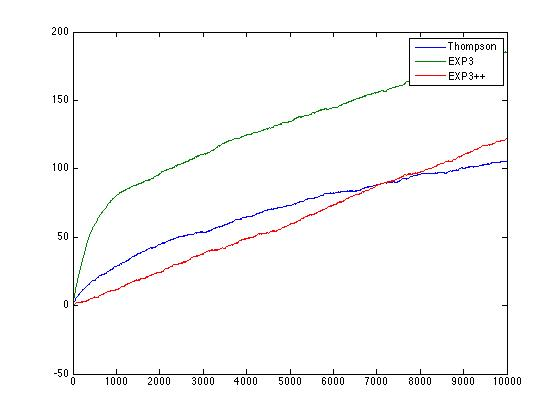
\includegraphics[width=\linewidth]{comparaison_contamined.jpg}
  \subcaption{5 stochastic and 5 adversarial arms}\label{fig:awesome_image1}
\endminipage\hfill
\minipage{0.33\textwidth}
  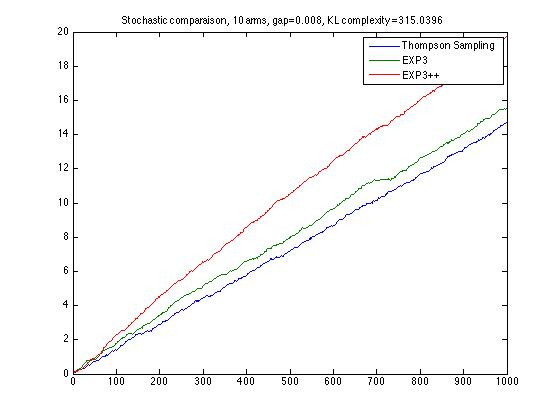
\includegraphics[width=\linewidth]{stochasticComparaison.jpg}
  \subcaption{Stochastic configuration with 10 arms}\label{fig:awesome_image2}
\endminipage\hfill
\minipage{0.33\textwidth}%
  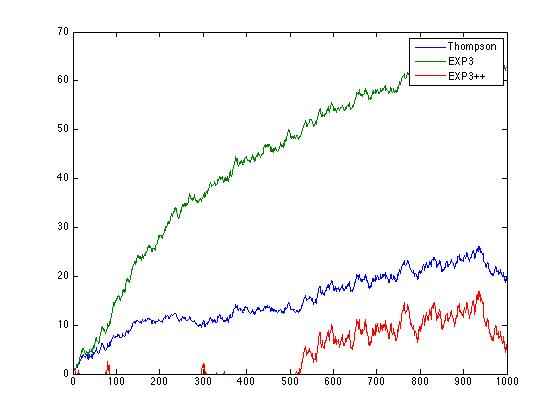
\includegraphics[width=\linewidth]{compAdversarial.jpg}
  \subcaption{Adversarial configuration}\label{fig:awesome_image3}
\endminipage
\caption{EXP3++ regret comparison}
\end{figure} 

As has already been stated in the paper, the EXP3++ algorithm indeed turns out to be rather effective in a contaminated environment. In the stochastic case, its performance is similar to the one of Thompson sampling. In the adversarial case, we see that the theoretical guarantee holds.


\pagebreak

\begin{thebibliography}{1}

\bibitem{Audi09} J.-Y. Audibert, R. Munos and C. Szepesvari (2009). {\em Exploration-exploitation tradeoff using variance estimates in multi-armed bandits}.  Theoretical Computer Science 410.19.

\bibitem{Audi10} J.-Y. Audibert and S. Bubeck (2010). {\em Regret bounds and minimax policies under partial monitoring}.  The Journal of Machine Learning Research 11.

\bibitem{Auer95} P. Auer, N. Cesa-Bianchi, Y. Freund and R.E. Schapire (1995). {\em Gambling in a rigged casino: The adversarial multi-armed bandit problem}. In Proceedings of the Annual Symposium on Foundations of Computer Science.

\bibitem{Auer02a} P. Auer, N. Cesa-Bianchi and P. Fischer (2002). {\em Finite-time analysis of the multiarmed bandit problem}. Machine Learning, 47.

\bibitem{Auer02b} P. Auer, N. Cesa-Bianchi, Y. Freund and R.E. Schapire (2002). {\em The nonstochastic multiarmed bandit problem}. SIAM Journal of Computing, 32(1).

\bibitem{Bube12} S. Bubeck and A. Slivkins (2012). {\em The best of both worlds: stochastic and adversarial bandits}. In Proceedings of the International Conference on Computational Learning Theory (COLT).

\bibitem{Cesa06} N. Cesa-Bianchi and G. Lugosi (2006). {\em Prediction, learning, and games}. Vol. 1. No. 1.1. Cambridge: Cambridge University Press.

\bibitem{Gari11} A. Garivier and O. Cappe (2011). {\em The KL-UCB algorithm for bounded stochastic bandits and beyond}. arXiv preprint arXiv:1102.2490.

\bibitem{Lai85} T.L. Lai and H. Robbins (1985). {\em Asymptotically efficient adaptive allocation rules}. Advances in Applied Mathematics, 6.

\bibitem{Robb52} H. Robbins (1952). {\em Some aspects of the sequential design of experiments}.  Bulletin of the American Mathematical Society.

\bibitem{Sani14} A. Sani, G. Neu and A. Lazaric (2014). {\em Exploiting easy data in online optimization}.  Advances in Neural Information Processing Systems.

\bibitem{Seld14} Y. Seldin and A. Slivkins (2014). {\em One practical algorithm for both stochastic and adversarial bandits}.  Proceedings of the 31st International Conference on Machine Learning (ICML-14).

\bibitem{Thom33} W.R. Thompson (1933). {\em On the likelihood that one unknown probability exceeds another in view of the evidence of two samples}. Biometrika, 25.

\end{thebibliography}

\pagebreak

\section*{Appendix}

\subsection*{The KL-UCB algorithm}
\begin{theorem}
Consider a bandit problem with K arms and independent rewards bounded in $[0, 1]$. Let $\epsilon > 0,$ and take $c = 3$. Let $a^*$ denote an arm with maximal expected reward $\mu_a$, and let $a$ be an arm such that $\mu_a < \mu_{a^*}$. For any positive integer $n$, the number of times algorithm KL-UCB chooses arm $a$ is upper-bounded by
$$ \mathbb{E}[N_{n}(a)] \leq \frac{\log n}{d(\mu_a, \mu_{a^*})}(1 + \epsilon) + C_1 \log(\log n) + \frac{C_2(\epsilon)}{n^{\beta(\epsilon)}},$$
where $C_1$ denotes a positive constant,  $C_2(\epsilon)$ and $\beta(\epsilon)$ positive functions of $\epsilon$ and $d(p,q)$ the KL divergence between Bernoulli distributions of parameters $p$ and $q$. Hence,
$$ \underset{n \rightarrow \infty}{\text{lim sup}} \; \frac{\mathbb{E}[N_{n}(a)]}{\log n} \leq \frac{1}{d(\mu_a, \mu_{a^*})}.$$
The regret of the KL-UCB algorithm then satisfies:
$$ \underset{n \rightarrow \infty}{\text{lim sup}} \; \frac{\mathbb{E}[R_n]}{\log n} \leq \sum_{a: \mu_a < \mu_{a^*}} \frac{\mu_a - \mu_{a^*}}{d(\mu_a, \mu_{a^*})}.$$
\end{theorem}

\subsection*{The EXP3 algorithm}

\begin{algorithm}[H]
\caption{EXP3}\label{EXP3}
Given fixed exploitation parameter $\eta$ and exploration parameter $\beta$\\
$\forall$ a $\omega_{a}(1)=1$\\
1. for t=2:$T_{end}$\\
2. $p_{a}(t) = (1-\beta)\frac{\omega_{a}(t-1)}{\sum_{a}\omega_{a}(t-1)}+\frac{\beta}{K}$\\
3. $A_{t}$ drawn with $p_{a}(t)$ distribution on arms\\
4. $\tilde{r}_{A_{t}} = \frac{r_{A_{t}}}{p_{A_{t}}(t-1)}$ and update of $\omega$ on $A_{t}$ only : $\omega_{A_{t}}(t)=\omega_{A_{t}}(t-1)exp(\eta \tilde{r}_{A_{t}(t)})$\\
\end{algorithm}

\subsection*{The EXP3++ algorithm}

\begin{algorithm}[H]
\caption{EXP3++}\label{EXP3++}
$\forall$ a $\tilde{L}_{0}(a)=0$\\
1. for $t=1:T_{end}$~\\
2. $\forall$ a $\in \{1,..K\}$\\
 $\epsilon_{t}(a)=min\{\frac{1}{2K}, \beta_{t}, \xi_{t}(a)\}$ \\
$\rho_{t}(a)=exp(-\eta_{t}\tilde{L}_{t-1}(a))/\sum_{a'}exp(-\eta_{t}\tilde{L}_{t-1}(a'))$\\
$\tilde{\rho}_{t}(a)=(1-\sum_{a'}\epsilon_{t}(a'))\rho_{t}(a)+\epsilon_{t}(a)$\\
3. Draw action $A_{t}$ with the $\tilde{\rho}_{t}$ distribution on arms.~\\
4. Observe the loss $l_{t}^{A_{t}}$ and $\forall$ a $\in \{1,..,K\}$\\
$\tilde{l}_{t}^{a}=\frac{l_{t}^{A_{t}}}{\tilde{\rho}_{t}(a)} \textbf{1}_{A_{t}=a}$\\
$\tilde{L}_{t}(a)=\tilde{L}_{t-1}(a)+\tilde{l}_{t}^{a}$
\end{algorithm}

\subsection*{The $(\mathcal{A},\, \mathcal{B})-$PROD algorithm for bandit problems}

\begin{minipage}{.5\textwidth}
  \begin{algorithm}[H] 
    \caption{$(\mathcal{A},\, \mathcal{B})-$PROD, Version 1} \label{Prod1}
    \textbf{Input:} learning rate $\eta \in (0, 1/2]$, initial weights $w_{1,\mathcal{A}} , w_{1,\mathcal{B} }$, num. of rounds $T$ ;\\
\textbf{For all} $t = 1, 2, ... , T$ \textbf{repeat} \\
1. Let $s_t = \frac{w_{t,\mathcal{A}}}{w_{t,\mathcal{A}} + w_{1,\mathcal{B}}} $\\
2. Observe $a_t$ and $b_t$ and predict
$$ x_t = \begin{cases}a_t&\text{with probability} s_t\\b_t&\text{otherwise}\end{cases}$$
3. Observe reward $f_t(x_t)$. \\
4. Update $\mathcal{A}$ and $\mathcal{B}$  with the (action, reward)-pairs $(a_t, \frac{f_t(x_t)}{s_t} \mathds{1}_{x_t = a_t})$ and $(b_t, \frac{f_t(x_t)}{1 - s_t} \mathds{1}_{x_t = b_t})$. \\
5. Compute $\delta_t = f_t(a_t) - f_t(b_t)$, where $f_t(a_t)$ and $f_t(b_t)$ are the rewards the algorithms have been updated with in step 4. Set
$$ w_{t+1} = w_t (1 + \eta \delta_t). $$
      \end{algorithm}
\end{minipage}%
\begin{minipage}{.5\textwidth}
  \begin{algorithm}[H]
    \caption{$(\mathcal{A},\, \mathcal{B})-$PROD, Version 2}  \label{Prod2}
    \textbf{Input:} learning rate $\eta \in (0, 1/2]$, initial weights $w_{1,\mathcal{A}} , w_{1,\mathcal{B} }$, num. of rounds $T$ ;\\
\textbf{For all} $t = 1, 2, ... , T$ \textbf{repeat} \\
1. Let $s_t = \frac{w_{t,\mathcal{A}}}{w_{t,\mathcal{A}} + w_{1,\mathcal{B}}} $\\
2. Observe $a_t$ and $b_t$ and predict
$$ x_t = \begin{cases}a_t&\text{with probability} s_t\\b_t&\text{otherwise}\end{cases}$$
3. Observe reward $f_t(x_t)$. \\
4. Update $\mathcal{A}$ and $\mathcal{B}$  both with the (action, reward)-pair $(x_t, f(x_t))$. \\
5. Compute $\delta_t = f_t(a_t) - f_t(b_t)$, where $f_t(a_t) = \frac{f_t(x_t)}{s_t} \mathds{1}_{x_t = a_t}$ and $f_t(b_t) = \frac{f_t(x_t)}{1 - s_t} \mathds{1}_{x_t = b_t}$ are unbiased estimators of the rewards. Set
$$ w_{t+1} = w_t (1 + \eta \delta_t). $$
  \end{algorithm}
\end{minipage}

=======
%----------------------------------------------------------------------------------------
%	PACKAGES AND OTHER DOCUMENT CONFIGURATIONS
%----------------------------------------------------------------------------------------

\documentclass[11pt]{article}
\usepackage{graphicx}
\usepackage[utf8]{inputenc}  
\usepackage[T1]{fontenc} 
\usepackage[top=1.4cm,bottom=1.2cm,left=1.3cm,right=2cm,asymmetric]{geometry}
\usepackage{amsfonts}
\usepackage{graphicx}
\usepackage{caption}
\usepackage{subcaption}
\usepackage{float}
\usepackage{subfig}
\usepackage{algorithm}
\usepackage{algpseudocode}
\usepackage{fancyhdr}
\usepackage{ stmaryrd }
\usepackage{placeins}
\usepackage{ amssymb }
\usepackage{mathtools}
\pagestyle{fancy}
\renewcommand{\footrulewidth}{1pt}
\fancyhead[R]{\textit{Master MVA : Reinforcement Learning}}
\fancyfoot[L]{\textit{}}
%\usepackage{unicode-math}
%\setmathfont{XITS Math}
%\setmathfont[version=setB,StylisticSet=1]{XITS Math}
\usepackage{array,multirow,makecell}
\setcellgapes{1pt}
\makegapedcells
\newcolumntype{R}[1]{>{\raggedleft\arraybackslash }b{#1}}
\newcolumntype{L}[1]{>{\raggedright\arraybackslash }b{#1}}
\newcolumntype{C}[1]{>{\centering\arraybackslash }b{#1}}

\pagestyle{fancy}
\renewcommand{\footrulewidth}{1pt}
\fancyfoot[L]{\textit{}}

\newcommand{\argmin}{\operatorname{arg min}}

\newtheorem{definition}{Definition}
\newtheorem{theorem}{Theorem}
\newtheorem{lemma}{Lemma}
\newtheorem{corollary}{Corollary}
\newtheorem{proposition}{Proposition}

\setlength{\parindent}{0pt}
   

\begin{document}

\parskip 6pt

\begin{center}
\section*{Final project - Reinforcement Learning}
\section*{Stochastic versus adversarial bandits}
\large{Isabella Joanna Lukasewitz \& Sammy Khalife}
\end{center}

\section*{Introduction}
Multi-armed bandit games are a simple model for sequential decision making that has been studied extensively from the second half of the last century on and that remains to be an important subject of research. The basic framework presents a player in a situation of sequential decision making. After each decision (out of a discrete and finite decision set) he receives a feedback from the environment in the form of a reward (or loss). The crucial tradeoff faced is the one between \textit{exploration} and \textit{exploitation}: While exploring the possible decision arms in order not to take suboptimal decisions, he/she should exploit what is already known in the best possible way. The performance of a strategy is usually measured as the regret with respect to a certain benchmark where the benchmark is generally given by the best fixed strategy throughout the game (to be defined more precisely in different scenarios).

For a long time, two main frameworks have been considered in the literature, largely independently from each other. The stochastic case assumes fixed underlying distributions for the respective decision arms (\cite{Thom33}, \cite{Robb85}, \cite{Auer02a}). The more general and therefore more difficult adversarial case (\cite{Auer95},  \cite{Auer02b}) does not make such an assumption. Rewards are assumed to be generated entirely randomly and fully determined given a sequence of decisions ahead of the game (while being obviously unknown to the player).

For both scenarios, algorithms have been developed with optimal worst-case guarantees. In a stochastic environment, the UCB1 algorithm (\cite{Auer02a}) for instance attends a regret of $O(\log n)$ while in the adversarial case $O(\sqrt{n})$ is reached by EXP3 (\cite{Auer02b}) for bounded rewards. However, generally algorithms designed for the stochastic framework fail completely in the adversarial one while algorithms adapted to the adversarial framework do not manage to take advantage of the "nice" stochastic case. Moreover, no frameworks different from the "extreme" adversarial and stochastic one have been considered.

Attempts to combine the two have been made only recently. In this article we aim first to provide a short overview of the most popular algorithms considered until today, their performance and their regret guarantees. In the second part, we will analyze more closely two algorithms proposed for the two frameworks jointly, the SAO algorithm (Bubeck et al., 2012 \cite{Bube12}) and the so-called EXP3++ (Seldin et al, 2014 \cite{Seld14}). Finally, we will present an algorithm that was proposed recently by Sani et al. \cite{Sani14}. It has been developed for a more general decision problem with full feedback. We will adapt it to the bandit framework and test its performance therein.

\section*{Multi-armed bandit environments}
Let $r_{t}^{A_{t}}$ be the reward obtained at time $t$ by pulling arm $A_{t}$. We will consider four different environments, following in that Seldin et al. \cite{Seld14}. In all cases, rewards are assumed to be bounded in $[0,1]$. The expected regret to be minimized is a priori defined as the difference between the expected loss of the algorithm up to round $t$ and the expected loss of the best arm up to round $t$:
$$\mathbb{E}[R(t)]=\max_{a}\{ \sum_{s=1}^{t} \mathbb{E}[r_{s}^{a}]\}-\sum_{s=1}^{t} \mathbb{E}[r_{s}^{A_{s}}].$$
The expectation is taken over the possible randomness of the algorithm and loss generation model. 

In the \textbf{adversarial regime}, the rewards are generated by an ''unrestricted adversary'' (oblivious to the algorithm's actions). This is the most general case. The regret is a posteriori computed as the difference to the best fixed strategy in hindsight: 
$$ R(t)=\max_{a}\{ \sum_{s=1}^{t} r_{s}^{a} \}-\sum_{s=1}^{t} r_{s}^{A_{s}}.$$

In the \textbf{stochastic regime}, we suppose that the rewards are sampled independently with respect to a distribution that does not depend on time, then $\mathbb{E}[r_{s}^{a}]=\mu_{a}$, and the regret simplifies : 
$$\mathbb{E}[R(t)]=t\max_{a}\mu_{a}-\sum_{s=1}^{t} \mathbb{E}[r_{s}^{A_{s}}]$$
which can be written as
$$\mathbb{E}[R(t)]=\sum_{a}\mathbb{E}[N_{t}(a)]\Delta_{a}$$ 
where $\Delta(a)=(\max_{a'}\mu_{a'})-\mu_{a}$ and $N_{t}(a)$ is the number of time a has been pulled until time t.

Seldin et al. introduce two new frameworks that can be regarded as in between the aforementioned ones.

The first of them is called \textbf{adversarial regime with a gap}, which is an adversarial regime for which we suppose that there exists a round $\tau$ and an arm $a_{\tau}*$ such that for any $t \geq \tau$, $a_{\tau}*$ persists to be the best arm in hindsight for all rounds $t \geq \tau$, i.e $\forall \, t \geq \tau$,  $a_{\tau}* \in \argmin_{a'}(\sum_{s=1}^{t}l_{s}^{a'})$.

The \textbf{contamined stochastic regime} is a stochastic regime with adversarial elements. The adversary chooses some pairs $(t,a)$ (''locations'') before the game starts and assigns their rewards in an arbitrary way. The rest of the rewards are generated as in the stochastic framework.

\section*{Popular bandit algorithms - an overview}

In this section we will give a short overview of the algorithms treated in class and compare their performance on several bandit problems. Since a lot of this material has been already treated throughout the course, we will keep the presentation short. Please note that all of the algorithms can be found in Appendix A. 

\subsection*{Stochastic framework}

The stochastic framework was the first one to be treated in multi-armed bandit problems. The Thompson algorithm, a very efficient algorithm for problems following the stochastic assumption, was already proposed in 1933 but was to be rediscovered many decades later \cite{Thom33}. A very popular basic learning algorithm is the UCB algorithm proposed by Auer et al. in \cite{Auer02a}.

It has been shown that the UCB achieves an essentially optimal regret of $O(\log n)$ (it matches the Lai-Robbins lower bound up to logarithmic factors). We recall this fact in the following theorem.
\begin{theorem}
The expected regret of the UCB algorithm is bounded as
$$ \mathbb{E}[R(t)] = \sum_{a}\mathbb{E}[N_{t}(a)]\Delta_{a} <
 6 \sum_{a: \, \Delta_a > 0} \frac{\log t}{\Delta_a} + K (\frac{\pi^2}{3} + 1).$$
\end{theorem}



\subsection*{Adversarial framework}




\section*{"The best of both worlds": The SAO algorithm}

There has only been very recently attempts to overcome the distinction between the two aforementioned frameworks. The first one was made by Bubeck et al. in 2012 \cite{Bube12}, where they introduced the so-called SAO algorithm. This algorithm manages in a certain way to bridge the gap between the two worlds: It has a build-in mechanism to detect the framework the player is in. However, it does not explicitly leave room for scenarios that are not purely stochastic or purely non-stochastic. This further extension will be tackled by the EXP3++ algorithm in the following section.

The SAO algorithm starts off like a classical algorithm for the stochastic framework, interleaving an \textit{exploration} and an \textit{exploitation} phase. At the beginning, all arms are activated and are sampled with the same probability. In the course of the algorithm, more and more arms get gradually deactivated (their sampling probability decreases smoothly) and the remaining arms are sampled with steadily increasing probability. The algorithm thus moves gradually from an exploration to a exploitation strategy. At each point in time, certain consistency conditions are checked to ensure that the assumed stochastic framework holds. As soon as one of these conditions fails, the algorithm assumes an adversarial framework and switches to the EXP3.P algorithm. This algorithm, based directly on the EXP3 algorithm, was equally proposed in \cite{Auer02b}. It introduces a biased estimate of the cumulative gain and exhibits advantageous theoretical properties when deriving high-probability bounds.

An an important novelty, they mange to prove an $\tilde{O}(\sqrt{n})$ regret bound for the adversarial case and a $polylog(n)$ bound for the stochastic case, thus coming close to the theoretical performance bounds for the UCB and the EXP3 algorithm that we recalled in the previous section. Their main result reads as follows:
\begin{theorem}
There exists an algorithm SAO for the MAB problem such that:
\begin{enumerate}
\item[(a)] in the adversarial model, SAO achieves regret $\mathbb{E}[R_n] \leq O(\sqrt{nK} \log^{3/2}(n) \log K)$.
?\item[(b)] in the stochastic model, SAO achieves regret $\mathbb{E}[R_n] \leq O(K \log^{2}(n) \log K)$.\end{enumerate}
\end{theorem}

The details are stated in the following theorem. The algorithm (with the explanation of the parameters) can be found in the appendix.
\begin{theorem}
SAO with $\beta = n^4$ satisfies in the stochastic model:
$$ \mathbb{E}[R_n] \leq O \left (\frac{K \log(K) \log^2(n)}{\Delta} \right),$$
and in the adversarial model:
$$\mathbb{E}[R_n] \leq O(\log(K) \log^{3/2}(n) \sqrt{nK}).$$
More precisely, for any $\delta \in (0,1)$, with probability at least $1-\delta$, SAO with $\beta = 10Kn^3 \delta^{-1}$ satisfies in the stochastic model:
$$\bar{R}_n = \frac{260K (1 + \log K) \log^2(\beta)}{\Delta},$$
and in the adversarial model:
$$R_n = \leq 60(1 + \log K) (1 + \log n) \sqrt{nK \log(\beta) + 5 K^2 \log^2(\beta)} + 200K^2 \log^2(\beta).$$
\end{theorem}

\subsection*{Numerical experiments}

We have tested the performance of the algorithm in comparison to several standard algorithms that were brought up in the last section. To our knowledge, this has not been done before, mainly because Bubeck et al. state themselves that a practical implementation of the algorithm should encompass some enhancements like an extension to a mixed stochastic-adversarial environment. As expected, the performance does therefore not quite match the one of the benchmarks. In several examples, we can see however how the algorithm actually manages to bridge the gap better than the current standard.


\section*{An adapted EXP3 algorithm}

As a reminder, the EXP3 algorithm is made as follows : 
\FloatBarrier
\begin{algorithm}
\caption{EXP3}\label{RS}
Given fixed exploitation parameter $\eta$ and exploration parameter $\beta$\\
$\forall$ a $\omega_{a}(1)=1$\\
1. for t=2:$T_{end}$\\
2. $p_{a}(t) = (1-\beta)\frac{\omega_{a}(t-1)}{\sum_{a}\omega_{a}(t-1)}+\frac{\beta}{K}$\\
3. $A_{t}$ drawn with $p_{a}(t)$ distribution on arms\\
4. $\tilde{r}_{A_{t}} = \frac{r_{A_{t}}}{p_{A_{t}}(t-1)}$ and update of $\omega$ on $A_{t}$ only : $\omega_{A_{t}}(t)=\omega_{A_{t}}(t-1)exp(\eta \tilde{r}_{A_{t}(t)})$\\
\end{algorithm}
\FloatBarrier
~\\
The EXP3 algorithm (Auer et al., 2002) is very efficient for adversarial frameworks, but has some difficulties to adapt to every kind of problems. Below the regrets in a stochastic framework compared with one of the most efficient algorithm in this case (Thompson sampling) :
\begin{center} \textbf{Comparaison of Thompson and EXP3 on stochastic framework}\end{center}
 \begin{figure}[!h]
   \begin{minipage}[c]{0.5 \linewidth}
   \centering
    \captionsetup{justification=centering,margin=1cm}
      \includegraphics[width=9cm]{Thompson_vs_exp3.jpg}
      \caption{''Easy problem''\\KL complexity = 6.3 (6 arms) $\beta=0.01$, $\eta$=0.01}
   \end{minipage} \hfill
   \begin{minipage}[c]{0.5 \linewidth}
   \centering
   \captionsetup{justification=centering,margin=1cm}
      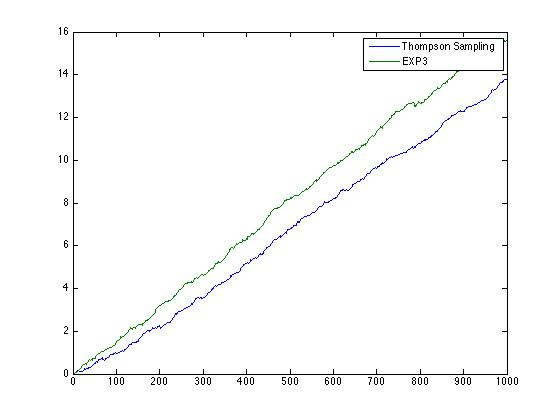
\includegraphics[width=9cm]{complexPbVs.jpg}
      \caption{''Difficult problem'',\\KL complexity = 315 (10 arms) $\beta$=0.01, $\eta$=0.01}
   \end{minipage} 
\end{figure}
~\\
To adapt EXP3 to stochastic configurations, the idea of the algorithm named EXP3++ (cf [1]) is to replace the exploration parameter $\beta$ and exploitation parameter $\eta$ by new time-depending parameters.
~\\
\FloatBarrier
\begin{algorithm}
\caption{EXP3++}\label{RS}
$\forall$ a $\tilde{L}_{0}(a)=0$\\
1. for $t=1:T_{end}$~\\
2. $\forall$ a $\in \{1,..K\}$\\
 $\epsilon_{t}(a)=min\{\frac{1}{2K}, \beta_{t}, \xi_{t}(a)\}$ \\
$\rho_{t}(a)=exp(-\eta_{t}\tilde{L}_{t-1}(a))/\sum_{a'}exp(-\eta_{t}\tilde{L}_{t-1}(a'))$\\
$\tilde{\rho}_{t}(a)=(1-\sum_{a'}\epsilon_{t}(a'))\rho_{t}(a)+\epsilon_{t}(a)$\\
3. Draw action $A_{t}$ with the $\tilde{\rho}_{t}$ distribution on arms.~\\
4. Observe the loss $l_{t}^{A_{t}}$ and $\forall$ a $\in \{1,..,K\}$\\
$\tilde{l}_{t}^{a}=\frac{l_{t}^{A_{t}}}{\tilde{\rho}_{t}(a)} \textbf{1}_{A_{t}=a}$\\
$\tilde{L}_{t}(a)=\tilde{L}_{t-1}(a)+\tilde{l}_{t}^{a}$
\end{algorithm}
\FloatBarrier~\\
With $\eta_{t}=2\beta_{t}$ and $\xi_{t}(a)=0$ we find back EXP3.


\section*{Theoretical results for EXP3++}
The main results have been demonstrated by Seldin et al. $[8]$.

\subsection*{Adversarial regimes}

\begin{theorem}
For $\eta_{t}=\beta_{t}$ and $\xi(t) \geq 0$, the regret for any $t\geq0$ satisfies $$R(t) \leq 4\sqrt{K\ln K}$$ This upper bound is two times above the EXP3 theoretical upper bound.
\end{theorem}

\subsection*{Stochastic regime}
First, if one supposes that we know the gaps, EXP3++ allows by defining adapted $\xi_{t}$ and $\eta_{t}$ to control the regret. In practice the gaps are not known and one will use an emprirical estimator : $$\hat{\Delta}_{t}(a)=min\{1,\frac{1}{t}(\max_{a'}(\tilde{L}_{t}(a')-\tilde{L}_{t}(a))\}$$
\begin{theorem}
Knowing the gaps $\Delta(a)$, with $\xi_{t}(a)=\frac{c\ln(t\Delta(a)^{2})}{t\Delta(a)^{2}}$, the regret satisfies :
$$R(t) \leq \sum_{a} O(\frac{\ln(t)^{2}}{\Delta(a)})+\sum_{a}\tilde{O}(\frac{K}{\Delta(a)^{3}})$$
\end{theorem}

\begin{theorem}
Let us consider the empirical gap $\Delta_{t}(a)$ defined previously, a time $t^{*}$ such that $t^{*}\geq \frac{4c^{2}K\ln(t*)^{4}}{\ln(K)}$ and let $t^{*}(a)=max\{t*,\lceil e^{1/\Delta(a)^{2}}\rceil\}$.
Then by tuning $\xi_{t}(a)=\frac{c\ln(t)^{2}}{t\hat{\Delta}_{t-1}(a)^{2}}$ (giving the EXP3$++^{AVG}$ algorithm) the regret in the stochastic regime satisfies :
$$R(t) \leq \sum_{a}O(\frac{\ln(t)^{3}}{\Delta{a}})+\sum_{a}\Delta(a)t^{*}(a)$$
\end{theorem}

\subsection*{Contamined stochastic regime}

\begin{theorem}
With the same assumptions as theorem 3 except $t^{*}(a)=max\{t^{*}, \lceil e^{4/\Delta(a)^{2}}\rceil \}$, the regret satisfies :
$$R(t) \leq \sum_{a}O(\frac{\ln(t)^{3}}{\Delta(a)})+\sum_{a}max\{t^{*}(a),\tau\}$$
\subsection*{Adversarial regime with a gap}
\textbf{Theorem 5} With the same assumptions as in theorem 3, the regret satisfies :
$$R(t) \leq \sum_{a}\{\min_{\tau}\{max\{t^{*},\tau,e^{1/(\Delta(\tau,a))^{2}}\}+O(\frac{\ln(t)^{3}}{\Delta(\tau,a)})\}$$~\\
\end{theorem}

With $\eta_{t}=\beta_{t}$, the EXP3++ algorithm provides a guarantee against adversarial situations. On the other hand, a configuration such that $\eta=1$ provide better results on a stochastic configuration. Still a lot has to be done concerning this trade-off.

\section*{Numerical comparison}
\subsection*{Comparison in a contaminated regime}
The comparison has been made with an implementation of EXP3++ with a time-depending gap $$\Delta(t,a)=\max_{a}(\mathbb{E}[r_{t}^{a}]-\mathbb{E}[r_{t}^{a}])$$ with 100 repetitions (Monte Carlo Simulations), the tuning  $\eta_{t}=\beta_{t}=\frac{1}{2}\sqrt{\frac{\ln(K)}{tK}}$ (Empirical EXP3++, cf [8]). The EXP3++ algorithm revealed to be more efficient on a contamined regime.
\begin{figure}[!h]
   \begin{minipage}[c]{0.5 \linewidth}
   \centering
    \captionsetup{justification=centering,margin=1cm}
      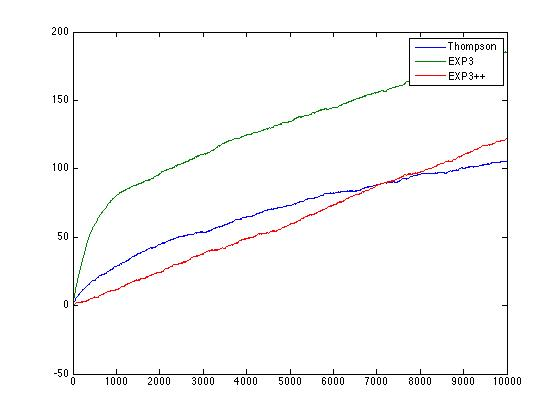
\includegraphics[width=10cm]{comparaison_contamined.jpg}
      \caption{Regret of EXP3 and EXP3++ algorithm on a contamined configuration with 5 stochastic arms and 5 adversarial arms}
   \end{minipage} \hfill
\end{figure}~\\

\newpage
\subsection*{Pure stochastic comparison}
\begin{figure}[!h]
	\begin{minipage}[c]{0.5 \linewidth}
		\centering
		\captionsetup{justification=centering,margin=1cm}
		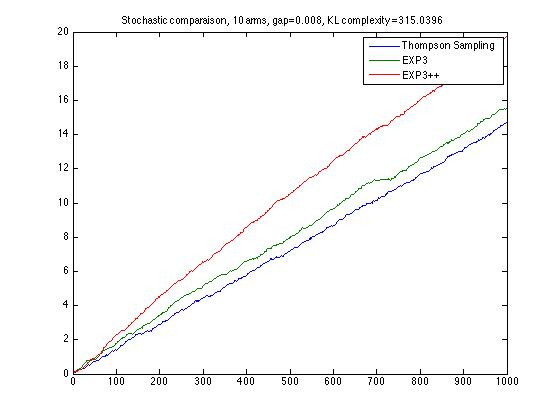
\includegraphics[width=10cm]{stochasticComparaison.jpg}
		\caption{Regret of EXP3 and EXP3++ algorithm on a stochastic configuration with 10 arms, KL complexity = 315}
	\end{minipage} \hfill
\end{figure}~\\
With the same tuning of parameters as previously for the EXP++ algorithm, its performance is equivalent to Thompson sampling.
\subsection*{Adversarial regime}
The advantage of EXP3++ is the guarantee for adversarial configurations, as we can see in the following comparison :
\begin{figure}[!h]
	\begin{minipage}[c]{0.5 \linewidth}
		\centering
		\captionsetup{justification=centering,margin=1cm}
		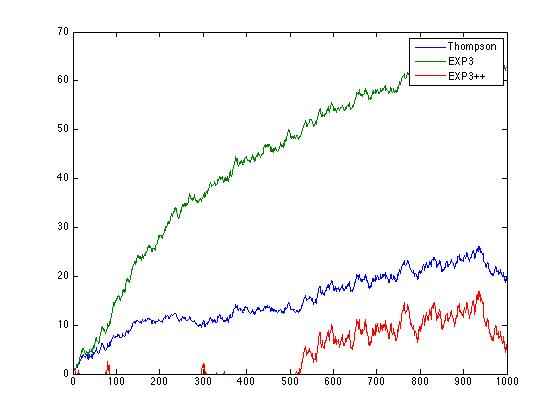
\includegraphics[width=10cm]{compAdversarial.jpg}
		\caption{Regret of three methods on adversarial configuration : 5 arms, $\eta_{t}=\beta_{t}$, $\xi_{t}=\frac{c\ln(t\Delta_{a,t}^{2})}{t\Delta_{a}^{2}}$}
	\end{minipage} \hfill
\end{figure}~\\

\subsection*{The $(\mathcal{A},\, \mathcal{B})-$PROD algorithm applied to multi-armed bandits}

The multi-armed bandit problem is a special case of a general online decision-making problem. It belongs to the class of partial feedback problems: In an MAB, the player's feedback is equal to his reward. He does in particular not obtain any knowledge regarding the theoretical rewards of the arms he has not played.

\pagebreak

\begin{thebibliography}{1}

\bibitem{Auer95} P. Auer, N. Cesa-Bianchi, Y. Freund and R.E. Schapire (1995). {\em Gambling in a rigged casino: The adversarial multi-armed bandit problem}. In Proceedings of the Annual Symposium on Foundations of Computer Science.

\bibitem{Auer02a} P. Auer, N. Cesa-Bianchi and P. Fischer (2002). {\em Finite-time analysis of the multiarmed bandit problem}. Machine Learning, 47.

\bibitem{Auer02b} P. Auer, N. Cesa-Bianchi, Y. Freund and R.E. Schapire (2002). {\em The nonstochastic multiarmed bandit problem}. SIAM Journal of Computing, 32(1).

\bibitem{Bube12} S. Bubeck and A. Slivkins (2012). {\em The best of both worlds: stochastic and adversarial bandits}. In Proceedings of the International Conference on Computational Learning Theory (COLT).

\bibitem{Lai85} T.L. Lai and H. Robbins (1985). {\em Asymptotically efficient adaptive allocation rules}. Advances in Applied Mathematics, 6.

\bibitem{Robb52} H. Robbins (1952). {\em Some aspects of the sequential design of experiments}.  Bulletin of the American Mathematical Society.

\bibitem{Sani14} A. Sani, G. Neu and A. Lazaric (2014). {\em Exploiting easy data in online optimization}.  Advances in Neural Information Processing Systems.

\bibitem{Seld14} Y. Seldin and A. Slivkins (2014). {\em One practical algorithm for both stochastic and adversarial bandits}.  Proceedings of the 31st International Conference on Machine Learning (ICML-14).

\bibitem{Thom33} W.R. Thompson (1933). {\em On the likelihood that one unknown probability exceeds another in view of the evidence of two samples}. Biometrika, 25.

\end{thebibliography}

>>>>>>> FETCH_HEAD
\end{document}